\chapter{Implementation} 
\label{chapter:implementation}
This chapter describes the implementation of Ethereum blockchain smart contracts and defines relationships between users and organizations.
//Blockchain node: fullnode.

\begin{figure}[hb]
    \centering
    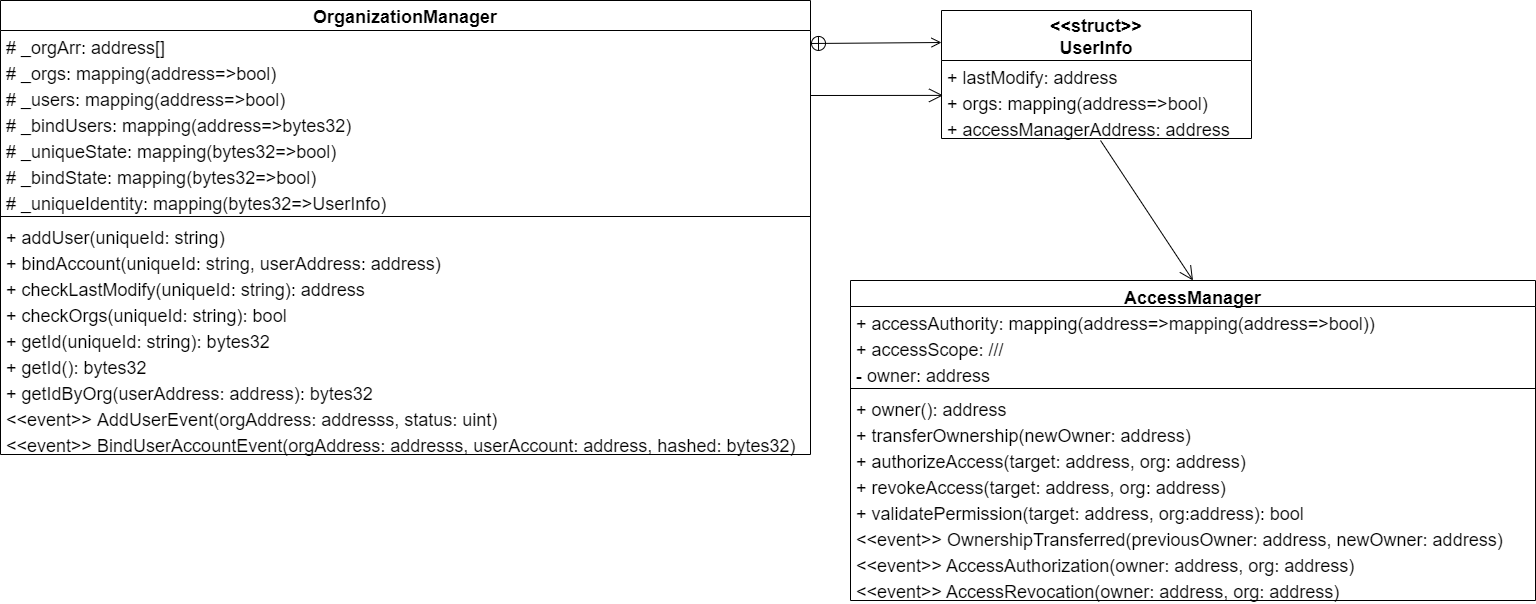
\includegraphics[height=!,width=1\linewidth,keepaspectratio=true]{figures/smart_contract_diagram.png}
    \caption{{\footnotesize Smart Contract Diagram}}
    \label{fig:smart_contract_diagram}
\end{figure}
\section{Smart contract design}
\subsection*{Organization Manager}
Each organization manages mapping of user and orgs.
// data structure
\subsection*{Access Manager}
Each user manages access control list of data.
// data structure

\section{Third Party Login}
\section{Integration Account}
\section{Data Sharing}
\section{Token design}
// jwt format